\documentclass[12pt]{beamer}
\setbeamertemplate{navigation symbols}


\setbeamerfont{institute}{size=\normalfont}
\usetheme{Madrid}

\usecolortheme{beaver}
\usepackage{graphicx}
\usepackage{tikz}
\usepackage{multirow}
% \usepackage{xcolor}
\definecolor{ashgrey}{rgb}{0.7, 0.75, 0.71}
\definecolor{gold}{HTML}{FFD700}
\definecolor{darkgold}{HTML}{8C7853}
\definecolor{darkseagreen}{HTML}{8FBC8F}
%%\usepackage[dvipsnames]{xcolor}


%Information to be included in the title page:

\author[ASA, LANA, SMRP]{Arnob Saha Ankon (1905108)\\Labid Al Nahiyan (1905110)\\SMR Pial (1905112)}

\institute
{
  Department of Computer Science and Engineering\\
  Bangladesh University of Engineering and Technology\\
}

\begin{document}
\title[TSP] %optional
{Traveling Salesman Problem}
\subtitle{
  CSE300 : Technical Writing and Presentation}


\logo{
\includegraphics[height=.75cm]{buet.png}}


\frame{\titlepage}



    
%%%%%%%%%%%%%%%%



\section{Let's look at TSP}
  \frametitle{The Traveling Salesman Problem}

 \begin{frame}{Travelling Salesman Problem}
 \begin{block}{Definition}
    The Traveling Salesman Problem (TSP) is a classic problem in computer science.Given a list of cities and the distances between them,We have to find out shortest possible route that visits each city exactly once and returns to the starting city
  \end{block}
\end{frame}


\begin{frame}{Example}
    Suppose we have three cities and a list of distances between each pair of cities. To find the shortest possible route by visiting each city- \pause
    \centering
    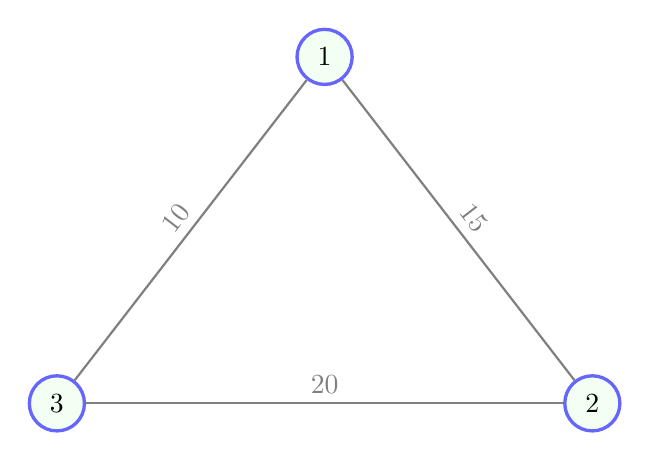
\begin{tikzpicture}[
        roundnode/.style={circle, draw=blue!60, fill=green!5, very thick, minimum size=7mm},
        ]
        \node[roundnode]  at(0,1) (1) {1};;
        \node[roundnode]  at(3.4,-3.4) (2) {2};
        \node[roundnode]  at(-3.4,-3.4) (3) {3};\pause;
        
        \draw[-,,gray, thick] (1)  -- node[sloped,above] {$10$}   (3) ; 
        \draw[-,gray,thick] (1) -- node[sloped,above] {$15$} (2);
        \draw[-,gray, thick] (2) -- node[sloped,above] {$20$}  (3);
       \end{tikzpicture}
\end{frame}

\begin{frame}
\frametitle{Example}


\centering
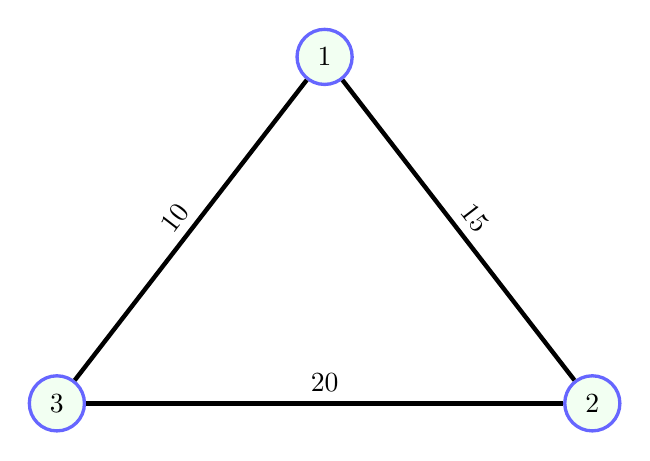
\begin{tikzpicture}[
roundnode/.style={circle, draw=blue!60, fill=green!5, very thick, minimum size=7mm},
]
\node[roundnode]  at(0,1) (Salesman) {1};
\node[roundnode]  at(3.4,-3.4) (city1) {2};
\node[roundnode]  at(-3.4,-3.4) (city2) {3};

\draw[-, ultra thick] (Salesman)  -- node[sloped,above] {$10$} (city2) ; 
\draw[-, ultra thick] (Salesman) -- node[sloped,above] {$15$} (city1);
\draw[-, ultra thick] (city1) -- node[sloped,above] {$20$} (city2);

\end{tikzpicture}
\end{frame}

\begin{frame}{Example}
    \centering
     \begin{exampleblock}{It is a very easy problem,isn't it?} 
        \pause
        But what happens if we have more nodes?
     \end{exampleblock}
\end{frame}

\begin{frame}{What if}

    \begin{columns}
        \column{.3\textwidth}
            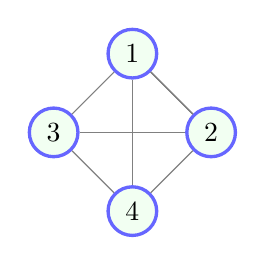
\begin{tikzpicture}[
        roundnode/.style={circle, draw=blue!60, fill=green!5, very thick, minimum size=4mm},
        ]
            \node[roundnode]  at(0,1) (1) {1};
            \node[roundnode]  at(1,0) (2) {2};
            \node[roundnode]  at(-1,0) (3) {3};
            \node[roundnode]  at(0,-1) (4) {4};

            \draw[-,,gray, thin] (1)  --  (2) ; 
            \draw[-,,gray, thin] (1)  --  (3) ; 
            \draw[-,,gray, thin] (1)  --  (4) ; 
            \draw[-,,gray, thin] (2)  --  (3) ; 
            \draw[-,,gray, thin] (3)  --  (4) ; 
            \draw[-,,gray, thin] (2)  --  (4) ; 
            \draw[-,,gray, thin] (1)  --  (2) ; 
            \draw[-,,gray, thin] (1)  --  (2) ; 
                
            \end{tikzpicture}
            
         \column{.3\textwidth}
            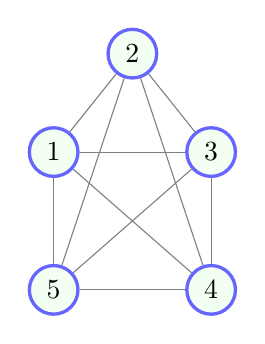
\begin{tikzpicture}[
        roundnode/.style={circle, draw=blue!60, fill=green!5, very thick, minimum size=4mm},
        ]
                \node[roundnode]  at(-1,.75) (1) {1};
                \node[roundnode]  at(0,2) (2) {2};
                \node[roundnode]  at(1,0.75) (3) {3};
                \node[roundnode]  at(1,-1)  (4) {4};
                \node[roundnode]  at(-1,-1) (5) {5};

                \draw[-,,gray, thin] (1)  --  (2) ; 
                \draw[-,,gray, thin] (1)  --  (3) ; 
                \draw[-,,gray, thin] (1)  --  (4) ; 
                \draw[-,,gray, thin] (1)  --  (5) ; 
                \draw[-,,gray, thin] (2)  --  (3) ; 
                \draw[-,,gray, thin] (2)  --  (4) ; 
                \draw[-,,gray, thin] (2)  --  (5) ; 
                \draw[-,,gray, thin] (3)  --  (4) ; 
                \draw[-,,gray, thin] (3)  --  (5) ; 
                \draw[-,,gray, thin] (4)  --  (5) ;
                
            \end{tikzpicture}
            
         \column{.3\textwidth}
            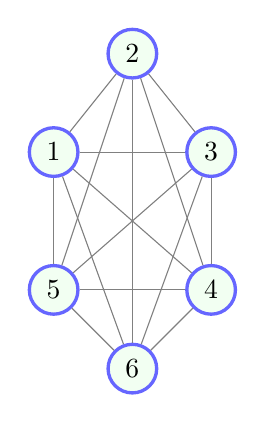
\begin{tikzpicture}[
        roundnode/.style={circle, draw=blue!60, fill=green!5, very thick, minimum size=5mm},
        ]
                \node[roundnode]  at(-1,.75) (1) {1};
                \node[roundnode]  at(0,2) (2) {2};
                \node[roundnode]  at(1,0.75) (3) {3};
                \node[roundnode]  at(1,-1) (4) {4};
                \node[roundnode]  at(-1,-1) (5) {5};
                \node[roundnode]  at(0,-2) (6) {6};

                \draw[-,,gray, thin] (1)  --  (2) ; 
                \draw[-,,gray, thin] (1)  --  (3) ; 
                \draw[-,,gray, thin] (1)  --  (4) ; 
                \draw[-,,gray, thin] (1)  --  (5) ; 
                \draw[-,,gray, thin] (1)  --  (6) ; 
                \draw[-,,gray, thin] (2)  --  (3) ; 
                \draw[-,,gray, thin] (2)  --  (4) ; 
                \draw[-,,gray, thin] (2)  --  (5) ;
                \draw[-,,gray, thin] (2)  --  (6) ; 
                \draw[-,,gray, thin] (3)  --  (4) ; 
                \draw[-,,gray, thin] (3)  --  (5) ; 
                \draw[-,,gray, thin] (3)  --  (6) ; 
                \draw[-,,gray, thin] (4)  --  (5) ; 
                \draw[-,,gray, thin] (4)  --  (6) ; 
                \draw[-,,gray, thin] (5)  --  (6) ;
                
            \end{tikzpicture}
            
    \end{columns}
    \pause
    {Now it is not so easy as before...}
\end{frame}

\begin{frame}{Think...}
    \begin{block}{ }
        If we have 'n' vertices then?\\
        \pause 
        We should find a general approach...
    \end{block}
\end{frame}

\begin{frame}{Brute force solution}
    \begin{columns}
        \column{.5\textwidth}
            \uncover<1->{When we have \alert{n} vertices\\} 
            \uncover<2->{For first vertex, we have  \alert{n} option\\}
            \uncover<3->{For second,we have \alert{(n-1)} option\\}
            \uncover<4->{...     ......    ....    ..   ..  ...   ......\\
            ...  ......    ....    ..   ..  ...   ......\\
            ...  ......    ....    ..   ..  ...   ......\\
            ...  ......    ....    ..   ..  ...   ......\\}
            \uncover<5->{For last vertex, we have \alert{1} option}
            
        \column{.5\textwidth}
           \uncover<2->{\Large\alert{$n$}}
           \uncover<3->{\Large\alert{$(n-1)$}}
           \uncover<4->{\Large \alert{$(n-2)$}}
           \uncover<5->{\Large\alert{$......$}}
           \uncover<6->{\Large\alert{$3.2.1$}}
           \newline
           \uncover<7->{\Large\alert{$=n!$}}
    \end{columns}
    
\end{frame}

\begin{frame}{Brute Force Time Complexity}
    \begin{alertblock}{}
        Time Complexity is O(n!) !!! \\
        What to do?
    \end{alertblock}
\end{frame}
%%%%%%%



\begin{frame}{Let's dive into TSP}
  \begin{itemize}
    \item<1-3> Actually, TSP is an NP-hard problem and finding an optimal solution using brute force is impractical for real-world applications.
    \item<2-3>  As the number of nodes increases, the problem becomes even more challenging.
    \item<3> Despite its computational complexity, TSP has numerous real-world applications, including logistics, transportation routing, network optimization, and circuit design.    
  \end{itemize}
  
\end{frame}

\begin{frame}{What to do?}
\begin{block}{So?}
    We need a solution!
\end{block}
    
\end{frame}

\begin{frame}{It's one of the hardest problem!}
    
  \begin{alertblock}{ }
    Even after several decades of extensive research, the Traveling Salesman Problem is still unsolved and there is no known algorithm that can efficiently solve all of its instances.
    \newline
    \newline
    It indicates the complexity and difficulty of this challenging computational problem!!!
  \end{alertblock}

\end{frame}


\begin{frame}{Exploring Alternative Solutions}
    \begin{block}{ }
     Upon realizing that our current approach may not yield the desired results, it is important to explore alternative solutions. Let us consider different options to overcome this challenge.
    \end{block}
\end{frame}


\begin{frame} {Exploring Alternative Solutions}

Here are some potential solutions-

    \begin{itemize}
        \item <1-> Exact Algorithms
        \item <2-> Heuristic Algorithms
        \item <3-> Metaheuristic Algorithms
        \item <4> ...
    \end{itemize}
  \end{frame}

  \begin{frame}      
  
  \begin{block}{Exact Algorithms}
   Exact algorithms offer a guaranteed optimal solution for TSP, but they can be computationally expensive, particularly for large problem sizes. \\
   Some of the popular exact algorithms for TSP 
    \begin{itemize}
      \item Dynamic programming\pause
      \item Branch and bound \pause
      \item ...
    \end{itemize}
  \end{block}

\end{frame}

 \begin{frame}

  \begin{block}{Heuristic Algorithms}
     Alternatively, heuristic algorithms offer a faster way to find good solutions for TSP. But they do not guarantee an optimal solution.
    Popular Heuristic algorithms:
    \begin{itemize}
    \item Greedy Algorithm \pause
      \item Nearest Neighbor \pause
      \item 2-opt solution\pause
      \item 3-opt solution \pause
      \item Christofides algorithms \pause\\ 
      \item ...
    \end{itemize}
  \end{block}
  % - (like kruskal)sort dep on, edge adding the possible lowest cost edge in each iteration
  
\end{frame}

% \begin{frame}
%   \begin{block}{Metaheuristic Algorithms}
%     Metaheuristic algorithms provide another approach to solving TSP and are applicable to a wide range of optimization problems. These algorithms utilize iterative processes to find good solutions and can be very effective for large problem sizes.
%     \\
%     Among the metaheuristic algorithms that have been applied to TSP, some of the popular ones are:
%     \begin{itemize}
%       \item Genetic algorithms \pause
%       \item Ant colony optimization\pause
%       \item ...
%     \end{itemize}
%   \end{block}
% \end{frame}      

 %%-Ant colony optimization is a population-based algorithm that simulates the behavior of ant colonies to efficiently search for good quality solutions to the Traveling Salesman Problem.

\begin{frame}{Selecting a feasible one}
    \begin{block}{ }
        Which one should we choose?
    \end{block}
\end{frame}
\begin{frame}{Comparison}
 
    \begin{tikzpicture}
    
        \tikzstyle{recleft} = [rectangle, rounded corners, minimum width=4.5cm, minimum height=0.75cm,text centered, draw=green!70, fill=green!5]    
        \tikzstyle{rect} = [rectangle, rounded corners, minimum width=3.5cm, minimum height=0.75cm,text centered, draw=green!70, fill=green!2.5]
        \tikzstyle{r} = [rectangle, rounded corners, minimum width=4.5cm, minimum height=0.75cm,text centered]
          \tikzstyle{r0} = [rectangle, rounded corners, minimum width=3.5cm, minimum height=0.75cm,text centered]
          
        \node (top) [r] {Algorithms};
        \node (mid) [r0, right of=top, xshift=3.5 cm] {Time complexity};
        \node (rig) [r0, right of=mid, xshift=2.5 cm] {Space complexity};
        \node (topLeft) [recleft, below of= top, yshift=0.25cm] {Brute Force};
        \node (topmid) [rect, right of=topLeft , xshift = 3.5cm] {$O(n!)$};
        \node (topright) [rect, right of=topmid , xshift = 2.5cm] {$O(n^2)$};
        
         \node (2ndLeft) [recleft, below of=topLeft, yshift=0.25cm] {Dynamic Programming};         
         \node (2ndmid) [rect, right of=2ndLeft , xshift = 3.5cm] {$O(n^2*2^n)$};
        \node (2ndright) [rect, right of=2ndmid, xshift =2.5cm] {$O(n^2)$};

         \node (3rdLeft) [recleft, below of=2ndLeft, yshift=0.25cm] {Branch & Bound};         
         \node (3rdmid) [rect, right of=3rdLeft , xshift = 3.5cm] {$O(n!)$};
        \node (3ndright) [rect, right of=3rdmid, xshift =2.5cm] {$O(n^2)$};

        \node (4Left) [recleft, below of=3rdLeft, yshift=0.25cm] {Nearest Neighbor};         
         \node (4mid) [rect, right of=4Left , xshift = 3.5cm] {$O(n^2)$};
        \node (4right) [rect, right of=4mid, xshift =2.5cm] {$O(n^2)$};

        \node (5Left) [recleft, below of=4Left, yshift=0.25cm] {2-Optimal Solution};         
         \node (5mid) [rect, right of=5Left , xshift = 3.5cm] {$O(n^2)$};
        \node (5right) [rect, right of=5mid, xshift =2.5cm] {$O(n^2)$};
        
         \node (6Left) [recleft, below of=5Left, yshift=0.25cm] {3-Optimal Solution};         
         \node (6mid) [rect, right of=6Left , xshift = 3.5cm] {$O(n^3)$};
        \node (6right) [rect, right of=6mid, xshift =2.5cm] {$O(n^2)$};

          \node (7Left) [recleft, below of=6Left, yshift=0.25cm] {Christrofides Algrothim};         
         \node (7mid) [rect, right of=7Left , xshift = 3.5cm] {$O(n^3)$};
        \node (7right) [rect, right of=7mid, xshift =2.5cm] {$O(n^2)$};

    \end{tikzpicture}
\end{frame}

\begin{frame}{Comparison}
    \begin{figure}[h]
        \centering
        \includegraphics[scale=0.2]{brute.png}
        \caption{Time (seconds) vs. the number of cities in a Traveling Salesman Problem for Brute force algorithm.
        \newline
        \newline
        \scriptsize{(https://scholarworks.calstate.edu/downloads/xg94hr81q)}}
        \label{fig:my_label}
        
    \end{figure}
\end{frame}

\begin{frame}{Comparison}
    \begin{figure}[h]
        \centering
        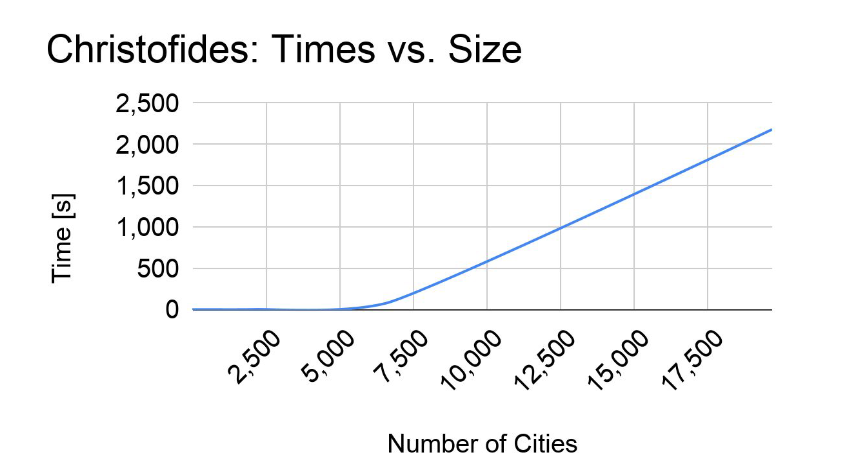
\includegraphics[scale=0.2]{chris.png}
       \caption{Time (seconds) vs. the number of cities in a Traveling Salesman Problem for Christofides algorithm.
        \newline
        \newline
        \scriptsize{(https://scholarworks.calstate.edu/downloads/xg94hr81q)}}
        \label{fig:my_label2}
    \end{figure}
\end{frame}
%%%%%%%



\begin{frame}{Approximate Solutions for Large TSP Problems}
Exact solutions to TSP can be expensive and impractical for real-life problems. Instead, approximate solutions like Christofides algorithm are often used which provides effective solutions for large TSP problem sizes.


%%%% PIAL ->

\end{frame}

\begin{frame}{Christofides Algorithm}
   \begin{columns}
   \begin{column}{0.5\textwidth}
    \begin{itemize}
        \item Christofides Algorithm is an approximate solution to the Traveling Salesman Problem (TSP).
        \item It was proposed by Nicos Christofides in 1976.
    \end{itemize}
    \end{column}
    \begin{column}{0.5\textwidth}
      \centering
      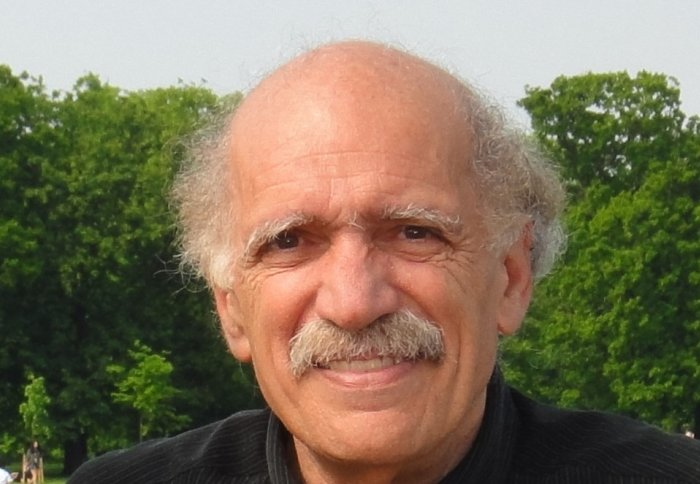
\includegraphics[width=5cm]{NC.jpg}\\
      Nicos Chrisrofides\\
      (1942-2019)
    \end{column}
    \end{columns}
\end{frame}
\begin{frame}{Christofides Algorithm (cont'd)}
\begin{itemize}
        \item The algorithm combines a minimum spanning tree with a matching algorithm to construct a solution that is guaranteed to be within a 1.5 times of the optimal solution.

\end{itemize}
\end{frame}
\begin{frame}{Christofides Algorithm (cont'd)}
    \begin{block}{Initial Graph}
    \begin{center}
    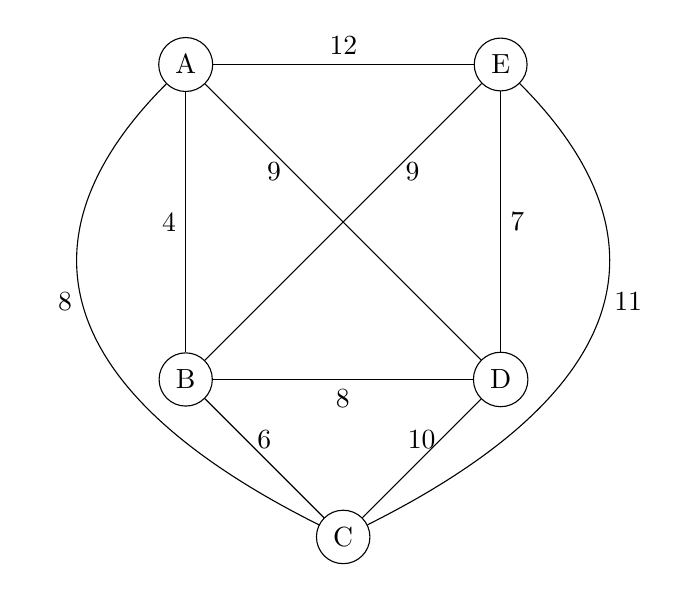
\begin{tikzpicture}
        \draw (0,0) node[circle,draw,scale=1] (B) {B};
        \draw (4,0) node[circle,draw,scale=1] (D) {D};
        \draw (0,4) node[circle,draw,scale=1] (A) {A};
        \draw (4,4) node[circle,draw,scale=1] (E) {E};
        \draw (2,-2) node[circle,draw,scale=1] (C) {C};
        \draw (A)--(B) node[left,pos=.5] {4};  
        \draw (A)--(D) node[below,pos=.25] {9};
        \draw (A)--(E) node[above,pos=.5] {12};
        \draw (B)--(C) node[above,pos=.5] {6};
        \draw (B)--(D) node[below,pos=.5] {8};
        \draw (B)--(E) node[below,pos=.75] {9};
        \draw (C)--(D) node[above,pos=.5] {10};      
        \draw (D)--(E) node[right,pos=.5] {7};

        \draw (A) .. controls (-2,2) and (-2,0) .. (C) node[left,pos=.5] {8};
        \draw (E) .. controls (6,2) and (6,0) .. (C)
        node[right,pos=.5] {11};
    \end{tikzpicture}
    \end{center}
    \end{block}
\end{frame}
\begin{frame}{Christofides Algorithm (cont'd)}
    \begin{itemize}
        \item The basic steps of the algorithm are as follows:
        \begin{enumerate}
          \item \textcolor{blue}{Find a minimum spanning tree (MST) of the input graph}.
        \end{enumerate}
    \end{itemize}
\end{frame}
\begin{frame}{Christofides Algorithm (cont'd)}
    \begin{block}{Minimum Spanning Tree}
    \begin{center}
    \begin{tikzpicture}
        \draw (0,0) node[circle,draw,scale=1] (B) {B};
        \draw (4,0) node[circle,draw,scale=1] (D) {D};
        \draw (0,4) node[circle,draw,scale=1] (A) {A};
        \draw (4,4) node[circle,draw,scale=1] (E) {E};
        \draw (2,-2) node[circle,draw,scale=1] (C) {C};
        \draw (A)--(B) node[left,pos=.5] {4};  
        \draw (B)--(D) node[below,pos=.5] {8};
        \draw (B)--(C) node[above,pos=.5] {6};     
        \draw (D)--(E) node[right,pos=.5] {7};
    \end{tikzpicture}
    \end{center}
    \end{block}
\end{frame}
\begin{frame}{Christofides Algorithm (cont'd)}
    \begin{itemize}
        \item The basic steps of the algorithm are as follows:
        \begin{enumerate}
          \item \textcolor{black}{Find a minimum spanning tree (MST) of the input graph}.
         \item \textcolor{blue}{Create a set of vertices with odd degree from the MST.}
        \end{enumerate}
    \end{itemize}
\end{frame}
\begin{frame}{Christofides Algorithm (cont'd)}
    \begin{block}{Odd Degree Vertices Of MST}
    \begin{center}
    \begin{columns}
        \begin{column}{0.45\textwidth}
        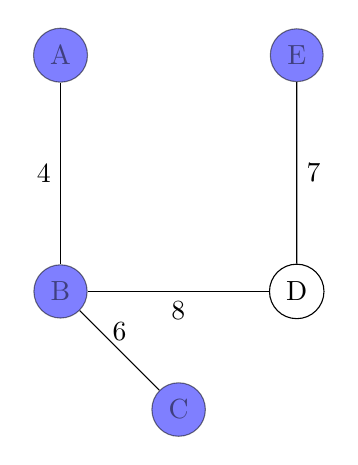
\begin{tikzpicture}[scale=.75]
            \draw (0,0) node[circle,draw,scale=1,
             fill=blue,opacity=.5] (B) {B};
            \draw (4,0) node[circle,draw,scale=1] (D) {D};
            \draw (0,4) node[circle,draw,scale=1,
            fill=blue,opacity=.5] (A) {A};
            \draw (4,4) node[circle,draw,scale=1,
             fill=blue,opacity=.5] (E) {E};
            \draw (2,-2) node[circle,draw,scale=1,
             fill=blue,opacity=.5] (C) {C};
            \draw (A)--(B) node[left,pos=.5] {4};  
            \draw (B)--(D) node[below,pos=.5] {8};
            \draw (B)--(C) node[above,pos=.5] {6};     
            \draw (D)--(E) node[right,pos=.5] {7};
        \end{tikzpicture}
        \end{column}
        \begin{column}{0.5\textwidth}
        Odd degree vertices are : A,B,C,E
        \end{column}
    \end{columns}
    \end{center}
    \end{block}
\end{frame}
\begin{frame}{Christofides Algorithm (cont'd)}
    \begin{itemize}
        \item The basic steps of the algorithm are as follows:
        \begin{enumerate}
          \item \textcolor{black}{Find a minimum spanning tree (MST) of the input graph}.
         \item \textcolor{black}{Create a set of vertices with odd degree from the MST.}
         \item \textcolor{blue}{Find a minimum-weight perfect matching on the set of vertices with odd degree.}
        \end{enumerate}
    \end{itemize}
\end{frame}
\begin{frame}{Christofides Algorithm (cont'd)}
    \begin{block}{Possible Perfect Matchings}
    \begin{center}
    \begin{columns}
        \begin{column}{0.5\textwidth}
            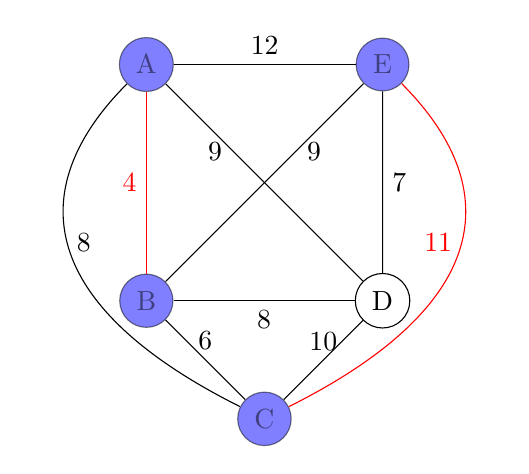
\begin{tikzpicture}[scale=.75]
             \draw (0,0) node[circle,draw,scale=1,
             fill=blue,opacity=.5] (B) {B};
            \draw (4,0) node[circle,draw,scale=1] (D) {D};
            \draw (0,4) node[circle,draw,scale=1,
            fill=blue,opacity=.5] (A) {A};
            \draw (4,4) node[circle,draw,scale=1,
             fill=blue,opacity=.5] (E) {E};
            \draw (2,-2) node[circle,draw,scale=1,
             fill=blue,opacity=.5] (C) {C};
            \draw[color=red] (A)--(B) node[left,pos=.5] {4};  
            \draw (A)--(D) node[below,pos=.25] {9};
            \draw (A)--(E) node[above,pos=.5] {12};
            \draw (B)--(C) node[above,pos=.5] {6};
            \draw (B)--(D) node[below,pos=.5] {8};
            \draw (B)--(E) node[below,pos=.75] {9};
            \draw (C)--(D) node[above,pos=.5] {10};      
            \draw (D)--(E) node[right,pos=.5] {7};
    
            \draw (A) .. controls (-2,2) and (-2,0) .. (C) node[right,pos=.5] {8};
            \draw[color=red] (E) .. controls (6,2) and (6,0) .. (C)
            node[left,pos=.5] {11};
            \end{tikzpicture}
        \end{column}
        \begin{column}{0.5\textwidth}
        Odd degree vertices are : A,B,C,E\\
         \vspace{.2cm}
        Possible perfect matching of these odd degree edges:\\
        \textcolor{red}{(A,B) + (C,E) = 4+11 = 15}\\
        \end{column}
    \end{columns}
    \end{center}
    \end{block}
\end{frame}
\begin{frame}{Christofides Algorithm (cont'd)}
    \begin{block}{Possible Perfect Matchings}
    \begin{center}
    \begin{columns}
        \begin{column}{0.5\textwidth}
            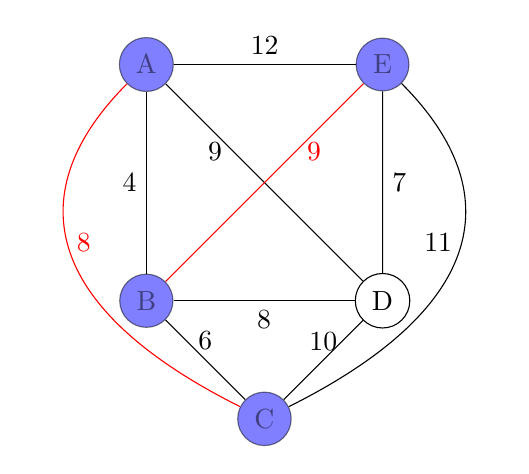
\begin{tikzpicture}[scale=.75]
             \draw (0,0) node[circle,draw,scale=1,
             fill=blue,opacity=.5] (B) {B};
            \draw (4,0) node[circle,draw,scale=1] (D) {D};
            \draw (0,4) node[circle,draw,scale=1,
            fill=blue,opacity=.5] (A) {A};
            \draw (4,4) node[circle,draw,scale=1,
             fill=blue,opacity=.5] (E) {E};
            \draw (2,-2) node[circle,draw,scale=1,
             fill=blue,opacity=.5] (C) {C};
            \draw (A)--(B) node[left,pos=.5] {4};  
            \draw (A)--(D) node[below,pos=.25] {9};
            \draw (A)--(E) node[above,pos=.5] {12};
            \draw (B)--(C) node[above,pos=.5] {6};
            \draw (B)--(D) node[below,pos=.5] {8};
            \draw[color=red] (B)--(E) node[below,pos=.75] {9};
            \draw (C)--(D) node[above,pos=.5] {10};      
            \draw (D)--(E) node[right,pos=.5] {7};
    
            \draw[color=red] (A) .. controls (-2,2) and (-2,0) .. (C) node[right,pos=.5] {8};
            \draw (E) .. controls (6,2) and (6,0) .. (C)
            node[left,pos=.5] {11};
            \end{tikzpicture}
        \end{column}
        \begin{column}{0.5\textwidth}
        Odd degree vertices are : A,B,C,E\\
         \vspace{.2cm}
        Possible perfect matching of these odd degree edges:\\
        (A,B) + (C,E) = 4+11 = 15\\
        \textcolor{red}{(A,C) + (B,E) = 8+9 = 17}\\

        \end{column}
    \end{columns}
    \end{center}
    \end{block}
\end{frame}
\begin{frame}{Christofides Algorithm (cont'd)}
    \begin{block}{Possible Perfect Matchings}
    \begin{center}
    \begin{columns}
        \begin{column}{0.5\textwidth}
            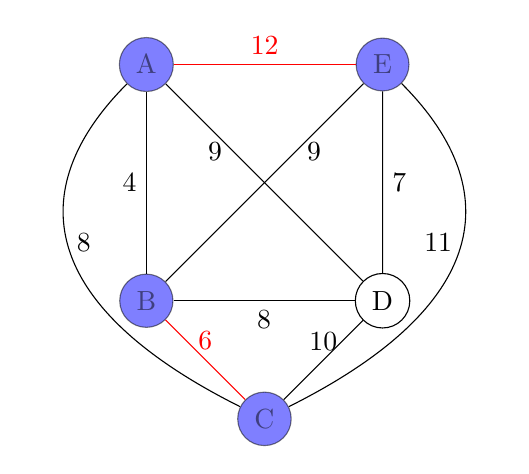
\begin{tikzpicture}[scale=.75]
             \draw (0,0) node[circle,draw,scale=1,
             fill=blue,opacity=.5] (B) {B};
            \draw (4,0) node[circle,draw,scale=1] (D) {D};
            \draw (0,4) node[circle,draw,scale=1,
            fill=blue,opacity=.5] (A) {A};
            \draw (4,4) node[circle,draw,scale=1,
             fill=blue,opacity=.5] (E) {E};
            \draw (2,-2) node[circle,draw,scale=1,
             fill=blue,opacity=.5] (C) {C};
            \draw (A)--(B) node[left,pos=.5] {4};  
            \draw (A)--(D) node[below,pos=.25] {9};
            \draw[color=red] (A)--(E) node[above,pos=.5] {12};
            \draw[color=red] (B)--(C) node[above,pos=.5] {6};
            \draw (B)--(D) node[below,pos=.5] {8};
            \draw (B)--(E) node[below,pos=.75] {9};
            \draw (C)--(D) node[above,pos=.5] {10};      
            \draw (D)--(E) node[right,pos=.5] {7};
    
            \draw (A) .. controls (-2,2) and (-2,0) .. (C) node[right,pos=.5] {8};
            \draw (E) .. controls (6,2) and (6,0) .. (C)
            node[left,pos=.5] {11};
            \end{tikzpicture}
        \end{column}
        \begin{column}{0.5\textwidth}
        Odd degree vertices are : A,B,C,E\\
         \vspace{.2cm}
        Possible perfect matching of these odd degree edges:\\
        (A,B) + (C,E) = 4+11 = 15\\
        (A,C) + (B,E) = 8+9 = 17\\
        \textcolor{red}{(A,E) + (B,C) = 12+6 = 18}\\

        \end{column}
    \end{columns}
    \end{center}
    \end{block}
\end{frame}
\begin{frame}{Christofides Algorithm (cont'd)}
    \begin{block}{Minimum Weight Perfect Matching}
    \begin{center}
    \begin{columns}
        \begin{column}{0.45\textwidth}
            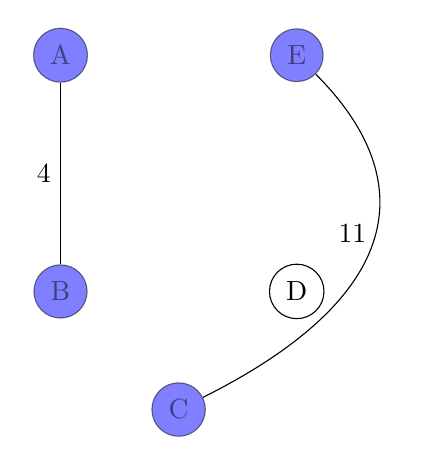
\begin{tikzpicture}[scale=.75]
             \draw (0,0) node[circle,draw,scale=1,
             fill=blue,opacity=.5] (B) {B};
            \draw (4,0) node[circle,draw,scale=1] (D) {D};
            \draw (0,4) node[circle,draw,scale=1,
            fill=blue,opacity=.5] (A) {A};
            \draw (4,4) node[circle,draw,scale=1,
             fill=blue,opacity=.5] (E) {E};
            \draw (2,-2) node[circle,draw,scale=1,
             fill=blue,opacity=.5] (C) {C};
            \draw (A)--(B) node[left,pos=.5] {4};  
            \draw (E) .. controls (6,2) and (6,0) .. (C)
            node[left,pos=.5] {11};
            \end{tikzpicture}
        \end{column}
        \begin{column}{0.5\textwidth}
        Odd degree vertices are : A,B,C,E\\
        \vspace{.2cm}
        Minimum perfect matching:\\
        (A,B) + (C,E) = 4+11 = 15\\
        \end{column}
    \end{columns}
    \end{center}
    \end{block}
\end{frame}
\begin{frame}{Christofides Algorithm (cont'd)}
    \begin{itemize}
        \item The basic steps of the algorithm are as follows:
        \begin{enumerate}
          \item \textcolor{black}{Find a minimum spanning tree (MST) of the input graph}.
         \item \textcolor{black}{Create a set of vertices with odd degree from the MST.}
         \item \textcolor{black}{Find a minimum-weight perfect matching on the set of vertices with odd degree.}
          \item \textcolor{blue} {Combine the edges from the MST and the minimum-weight perfect matching to form an Eulerian graph.}
        \end{enumerate}
    \end{itemize}
\end{frame}
\begin{frame}{Christofides Algorithm (cont'd)}
    \begin{block}{Minimum Perfect Matching vs MST}
    \begin{center}
    \begin{columns}
        \begin{column}{0.45\textwidth}
            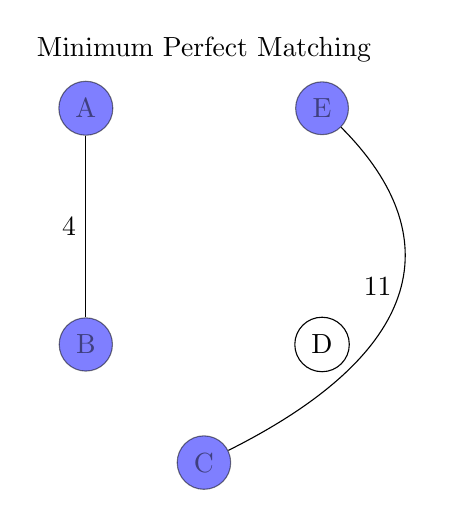
\begin{tikzpicture}[scale=.75]
            \draw (2,5) node[]{Minimum Perfect Matching};
            \draw (0,0) node[circle,draw,scale=1,
             fill=blue,opacity=.5] (B) {B};
            \draw (4,0) node[circle,draw,scale=1] (D) {D};
            \draw (0,4) node[circle,draw,scale=1,
            fill=blue,opacity=.5] (A) {A};
            \draw (4,4) node[circle,draw,scale=1,
             fill=blue,opacity=.5] (E) {E};
            \draw (2,-2) node[circle,draw,scale=1,
             fill=blue,opacity=.5] (C) {C};
            \draw (A)--(B) node[left,pos=.5] {4};  
            \draw (E) .. controls (6,2) and (6,0) .. (C)
            node[left,pos=.5] {11};
            \end{tikzpicture}
        \end{column}
        \begin{column}{0.50\textwidth}
        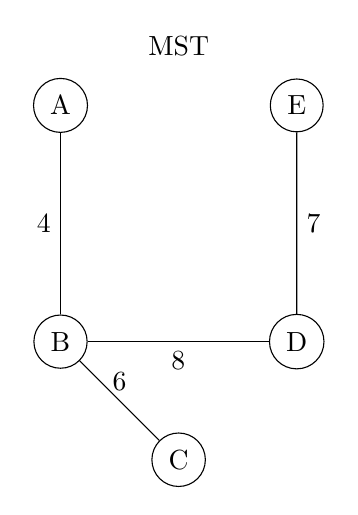
\begin{tikzpicture}[scale=.75]
        \draw (2,5) node[]{MST};
        \draw (0,0) node[circle,draw,scale=1] (B) {B};
        \draw (4,0) node[circle,draw,scale=1] (D) {D};
        \draw (0,4) node[circle,draw,scale=1] (A) {A};
        \draw (4,4) node[circle,draw,scale=1] (E) {E};
        \draw (2,-2) node[circle,draw,scale=1] (C) {C};
        \draw (A)--(B) node[left,pos=.5] {4};  
        \draw (B)--(D) node[below,pos=.5] {8};
        \draw (B)--(C) node[above,pos=.5] {6};     
        \draw (D)--(E) node[right,pos=.5] {7};
        \end{tikzpicture}
    \end{column}
    \end{columns}
    \end{center}
    \end{block}
\end{frame}
\begin{frame}{Christofides Algorithm (cont'd)}
    \begin{block}{MST+Minimum Perfect Macthing}
    \begin{center}
    \begin{tikzpicture}
        \draw (0,0) node[circle,draw,scale=1] (B) {B};
        \draw (4,0) node[circle,draw,scale=1] (D) {D};
        \draw (0,4) node[circle,draw,scale=1] (A) {A};
        \draw (4,4) node[circle,draw,scale=1] (E) {E};
        \draw (2,-2) node[circle,draw,scale=1] (C) {C};
        \draw (A)--(B) node[left,pos=.5] {4};  
        \draw[dashed] (A) .. controls (-1,3) and (-1,1) .. (B)
        node[left,pos=.5] {4};
        
        \draw (B)--(C) node[above,pos=.5] {6};
        \draw (B)--(D) node[below,pos=.5] {8};     
        \draw (D)--(E) node[right,pos=.5] {7};

        \draw[dashed] (E) .. controls (6,2) and (6,0) .. (C)
        node[left,pos=.5] {11};
    \end{tikzpicture}
    \end{center}
    \end{block}
\end{frame}
\begin{frame}{Christofides Algorithm (cont'd)}
    \begin{block}{Euler Circuit}
    \vspace{1cm}
    An Euler Circuit is a path that goes
    through every edge of a graph
    exactly once and begins and ends at
    the same vertex.
    \vspace{1cm}
    \end{block}
\end{frame}
\begin{frame}{Christofides Algorithm (cont'd)}
    \begin{block}{Euler Circuit Of Graph}
    \begin{center}
    \begin{columns}
    \begin{column}{0.5\textwidth}
        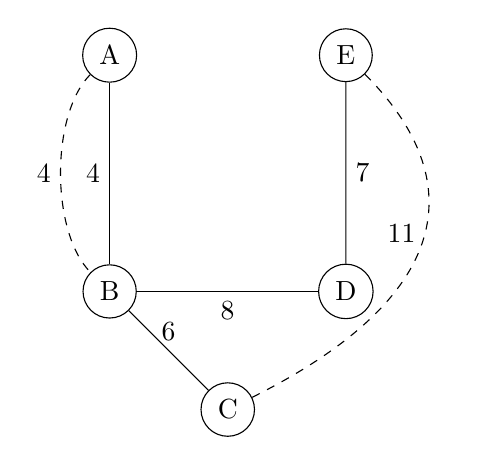
\begin{tikzpicture}[scale=0.75]
        \draw (0,0) node[circle,draw,scale=1] (B) {B};
        \draw (4,0) node[circle,draw,scale=1] (D) {D};
        \draw (0,4) node[circle,draw,scale=1] (A) {A};
        \draw (4,4) node[circle,draw,scale=1] (E) {E};
        \draw (2,-2) node[circle,draw,scale=1] (C) {C};
        \draw (A)--(B) node[left,pos=.5] {4};  
        \draw[dashed] (A) .. controls (-1,3) and (-1,1) .. (B)
        node[left,pos=.5] {4};
        
        \draw (B)--(C) node[above,pos=.5] {6};
        \draw (B)--(D) node[below,pos=.5] {8};     
        \draw (D)--(E) node[right,pos=.5] {7};

        \draw[dashed] (E) .. controls (6,2) and (6,0) .. (C)
        node[left,pos=.5] {11};
        \end{tikzpicture}
    \end{column}
    \begin{column}{0.5\textwidth}
    Here the euler circuit is:
    A-B-C-E-D-B-A
    \end{column}
    \end{columns}
    \end{center}
    \end{block}
\end{frame}
\begin{frame}{Christofides Algorithm (cont'd)}
 \begin{itemize}
        \item The basic steps of the algorithm are as follows:
        \begin{enumerate}
          \item \textcolor{black}{Find a minimum spanning tree (MST) of the input graph}.
         \item \textcolor{black}{Create a set of vertices with odd degree from the MST.}
         \item \textcolor{black}{Find a minimum-weight perfect matching on the set of vertices with odd degree.}
          \item \textcolor{black} {Combine the edges from the MST and the minimum-weight perfect matching to form an Eulerian graph.}
          \item \textcolor{blue}{Remove repeated vertices from the Eulerian circuit to obtain a Hamiltonian circuit, which is a valid tour of the cities.}
        \end{enumerate}
    \end{itemize}
\end{frame}
\begin{frame}{Christofides Algorithm (cont'd)}
    \begin{block}{Hamiltonian Circuit}
    \vspace{1cm}
    A Hamiltonian circuit is a path that visits every vertex once with no repeats. Being a circuit, it must start and end at the same vertex.
    \vspace{1cm}
    \end{block}
\end{frame}
\begin{frame}{Christofides Algorithm (cont'd)}
    \begin{block}{Eliminate Repetition}
    \begin{center}
    \begin{columns}
    \begin{column}{0.5\textwidth}
        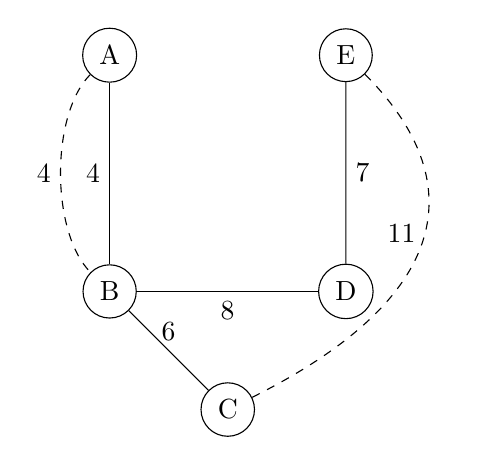
\begin{tikzpicture}[scale=0.75]
        \draw (0,0) node[circle,draw,scale=1] (B) {B};
        \draw (4,0) node[circle,draw,scale=1] (D) {D};
        \draw (0,4) node[circle,draw,scale=1] (A) {A};
        \draw (4,4) node[circle,draw,scale=1] (E) {E};
        \draw (2,-2) node[circle,draw,scale=1] (C) {C};
        \draw (A)--(B) node[left,pos=.5] {4};  
        \draw[dashed] (A) .. controls (-1,3) and (-1,1) .. (B)
        node[left,pos=.5] {4};
        
        \draw (B)--(C) node[above,pos=.5] {6};
        \draw (B)--(D) node[below,pos=.5] {8};     
        \draw (D)--(E) node[right,pos=.5] {7};

        \draw[dashed] (E) .. controls (6,2) and (6,0) .. (C)
        node[left,pos=.5] {11};
        \end{tikzpicture}
    \end{column}
    \begin{column}{0.5\textwidth}
    Eliminate repetition from the euler circuit.\\
    Here the euler circuit is:
    A-B-C-E-D-\textcolor{red}{B}-A\\
    \end{column}
    \end{columns}
    \end{center}
    \end{block}
\end{frame}
\begin{frame}{Christofides Algorithm (cont'd)}
    \begin{block}{Hamiltonian Circuit Of Graph}
    \begin{center}
    \begin{columns}
    \begin{column}{0.5\textwidth}
        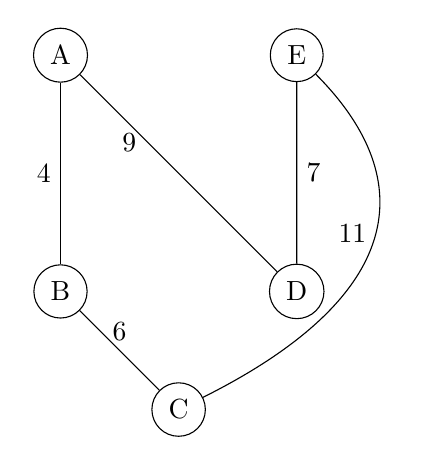
\begin{tikzpicture}[scale=0.75]
        \draw (0,0) node[circle,draw,scale=1] (B) {B};
        \draw (4,0) node[circle,draw,scale=1] (D) {D};
        \draw (0,4) node[circle,draw,scale=1] (A) {A};
        \draw (4,4) node[circle,draw,scale=1] (E) {E};
        \draw (2,-2) node[circle,draw,scale=1] (C) {C};
        \draw (A)--(B) node[left,pos=.5] {4};  
        \draw (B)--(C) node[above,pos=.5] {6};     
        \draw (D)--(E) node[right,pos=.5] {7};
        \draw (A)--(D) node[below,pos=.25] {9};
        \draw (E) .. controls (6,2) and (6,0) .. (C)
        node[left,pos=.5] {11};
        \end{tikzpicture}
    \end{column}
    \begin{column}{0.5\textwidth}
    After eliminating repetition the resulting graph becomes a hamiltonian circuit.\\
    Here the hamiltonian circuit is:
    A-B-C-E-D-A\\
    \end{column}
    \end{columns}
    \end{center}
    \end{block}
\end{frame}
\begin{frame}{Christofides Algorithm (cont'd)}
    \begin{block}{Hamiltonian Circuit Of Graph}
    \begin{center}
    \begin{columns}
    \begin{column}{0.5\textwidth}
        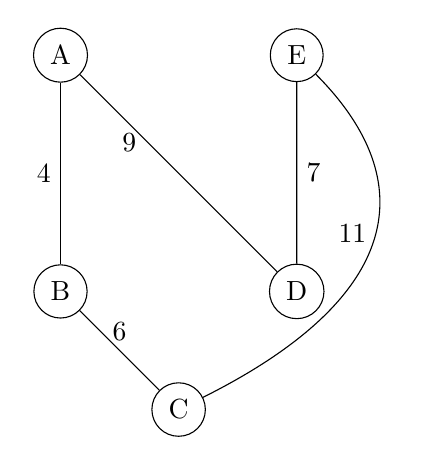
\begin{tikzpicture}[scale=0.75]
        \draw (0,0) node[circle,draw,scale=1] (B) {B};
        \draw (4,0) node[circle,draw,scale=1] (D) {D};
        \draw (0,4) node[circle,draw,scale=1] (A) {A};
        \draw (4,4) node[circle,draw,scale=1] (E) {E};
        \draw (2,-2) node[circle,draw,scale=1] (C) {C};
        \draw (A)--(B) node[left,pos=.5] {4};  
        \draw (B)--(C) node[above,pos=.5] {6};     
        \draw (D)--(E) node[right,pos=.5] {7};
        \draw (A)--(D) node[below,pos=.25] {9};
        \draw (E) .. controls (6,2) and (6,0) .. (C)
        node[left,pos=.5] {11};
        \end{tikzpicture}
    \end{column}
    \begin{column}{0.5\textwidth}
    This is a valid tour of the cities and our desired answer.\\
    Total weight = 4+6+7+9+11 = 37
    \end{column}
    \end{columns}
    \end{center}
    \end{block}
\end{frame}
% \begin{frame}{Christofides Algorithm (cont'd)}
%      \begin{block}{Complexity}
%      \vspace{1cm}
%     \hspace{.5cm} \textcolor{black}{Given n cities}
%     \begin{itemize}
%         \item \textcolor{ashgrey}{The time complexity of the algorithm is O($n^3$)}
%         \item \textcolor{ashgrey}{The space complexity of the algorithm is O($n^2$)}
%     \end{itemize} 
%     \vspace{1cm}
%     \end{block}
% \end{frame}
% \begin{frame}{Christofides Algorithm (cont'd)}
%     \begin{block}{Complexity}
%     \vspace{1cm}
%     \hspace{.5cm}  \textcolor{black}{Given n cities}
%     \begin{itemize}
%         \item \textcolor{black}{The time complexity of the algorithm is O($n^3$)}
%         \item \textcolor{ashgrey}{The space complexity of the algorithm is O($n^2$)}
%     \end{itemize}  
%     \vspace{1cm}
%     \end{block}
% \end{frame}
% \begin{frame}{Christofides Algorithm (cont'd)}
%      \begin{block}{Complexity} 
%      \vspace{1cm}
%      \hspace{.5cm}  \textcolor{black}{Given n cities}
%     \begin{itemize}
%         \item \textcolor{black}{The time complexity of the algorithm is O($n^3$)}
%         \item \textcolor{black}{The space complexity of the algorithm is O($n^2$)}
%     \end{itemize} 
%     \vspace{1cm}
%     \end{block}
% \end{frame}
\begin{frame}{1 Million Dollar Challenge}
    \vspace{1cm}
    \centering
    {\Large \textbf{\textcolor{brown}{Can You Solve the TSP Problem?}}}\\
    \vspace{.2cm}
    {\Large \textbf{\textcolor{darkseagreen}{Claim Your Prize of 1 Million Dollars!}}}\\
    \vspace{1cm}
    
\includegraphics[width=5cm]{CashBundle.jpg}
\end{frame}
\begin{frame}{References}
    \begin{enumerate}
        \item \url{https://www.slideshare.net/SubathraKishore/approximation-algorithms-tsp}
        \item
        \url{https://bochang.me/blog/posts/tsp/}
        \item 
        \url{https://en.wikipedia.org/wiki/Nicos_Christofides}
        \item \url{https://www.khanacademy.org/computing/ap-computer-science-principles/algorithms-101/solving-hard-problems/a/using-heuristics}
        \item \url{https://cs.stackexchange.com/questions/93185/time-complexity-of-travelling-salesman-problem}
        \item \url{https://stemlounge.com/animated-algorithms-for-the-traveling-salesman-problem/}
        \item     \url{https://developers.google.com/optimization/reference/graph/christofides\#:~:text=The\%20complexity\%20of\%20the\%20algorithm,number\%20of\%20edges\%20of\%20the}
    \end{enumerate}
\end{frame}
\end{document}